\documentclass[%
12pt, %
final, % 
oneside, % 
onecolumn, %  
centertags]{article} % относится к классу article и размер шрифта 12 пунктовб, {article: статья, report: отчеты и диссертации, book: книга, letter: письмо}

% \usepackage{fontspec}
 
% \setmainfont{Times New Roman}

% \documentclass[a4paper, 12pt]{report}

\topmargin= -30pt % насколько сверху будет страница
\textheight= 650pt


\usepackage[utf8]{inputenc} % задает кодировку, utf-8 кодировка, включающая в себя знаки почти всех языков мира
\usepackage[english]{babel} % подключает необходимые языки, основным языком является английский

\selectlanguage{english} % настройки будут на английском, но писать будет на русском

\usepackage{euscript}
\usepackage{supertabular}

\renewcommand{\baselinestretch}{1.0} 

\usepackage[colorlinks=true,linkcolor=blue,unicode=true,urlcolor = blue]{hyperref} %hypered
\usepackage[pdftex]{graphicx} % для графики

\usepackage{amsthm, amssymb, amsmath, amsfonts} % математический пакет, математические шрифты
\usepackage{textcomp}
\usepackage[noend]{algorithmic}
\usepackage[ruled]{algorithm}
\usepackage{lipsum}
\usepackage{indentfirst}
\usepackage{babel}
\usepackage{pgfplots}
\usepackage{setspace}
\usepackage{xcolor}
\usepackage{hyperref}
\usepackage{subfigure}

\setcounter{secnumdepth}{5}
\setcounter{tocdepth}{5}
\newcommand\simpleparagraph[1]{%
  \stepcounter{paragraph}\paragraph*{\theparagraph\quad{}#1}}
\usepackage{listings}
% \usepackage{xcolor}
%\usepackage{minted}

\lstset { %
     language=C++,
     backgroundcolor=\color{black!5}, % set backgroundcolor
     basicstyle=\footnotesize,% basic font setting
}


\linespread{1.0} 
\setlength{\parindent}{2.4em}
\setlength{\parskip}{0.1em}

\pgfplotsset{compat=1.9}
\pgfplotsset{model/.style = {blue, samples = 100}} 
\pgfplotsset{experiment/.style = {red}}

\theoremstyle{plain}
\binoppenalty=10000

\newtheorem{theorem}{Theorem}[section] % theorem

\theoremstyle{definition}
% \newtheorem{definition}{Определение}[subsection]
\newtheorem{definition}{Definition}[subsection]

\theoremstyle{remark}
% \newtheorem{remark}{Замечание}[section]

% \newtheorem{corollary}{Следствие}

% \newtheorem{proposition}{Proposition}

% \newtheorem{example}{Пример}

% \newtheorem{lemma}{Лемма}[section]

\renewcommand*{\proofname}{Proof}

\graphicspath{ {./images/} }


% \usepackage{amsmath,amsfonts,amssymb, setspace}  % Разнообразные математические команды и значки
% \usepackage{indentfirst}     % Отступ в первом абзаце

% \pagestyle{empty}
\usepackage[left=2.5cm, right=1.5cm, top=2.5cm, bottom=2.5cm]{geometry}
\usepackage[medium]{titlesec}
\usepackage{graphicx}
% \graphicspath{ {./images/} }

\begin{document}

	\begin{titlepage} 
		\begin{center}
		\textbf{}\\[2.0cm]
		\LARGE FEDERAL STATE AUTONOMOUS EDUCATIONAL INSTITUTION OF HIGHER EDUCATION \\[0.5cm]
		\Large ITMO UNIVERSITY \\[3cm]
		\LARGE Report\\
		\Large MPI. Assignments $9$, $10$, $11$ \\
		\Large Parallel algorithms for the analysis and synthesis of data \\[4cm]


		\begin{flushright}
		Performed by\\
		Aleksandr Shirokov\\
		J4133c\\
		Accepted by\\
		Petr Andriushchenko

		Deadline: 21.12.21
		\end{flushright}

		\vfill 

		{\Large {St. Petersburg}} \par
		{\Large {2021}}
		\end{center} 
	\end{titlepage}

\tableofcontents
\newpage


\section{Assignments}

\subsection{Assignment 9. MPI\_Reduce.}

\subsubsection{Formulation of the problem}

\subsubsection{Example of launch parameters and output. Detailed description of solution}

Code for \textbf{assignment 9} is \href{https:\//github.com/aptmess/parallel_algorithms/blob/master/HT/hw_mpi/Assignment8.c}{here}.

Compilation example: \textsc{mpic++ -o ./cpf/8.o Assignment8.c}

Launch example: \textsc{mpirun --oversubscribe -np 2 ./cpf/8.o}

% \begin{center}
% 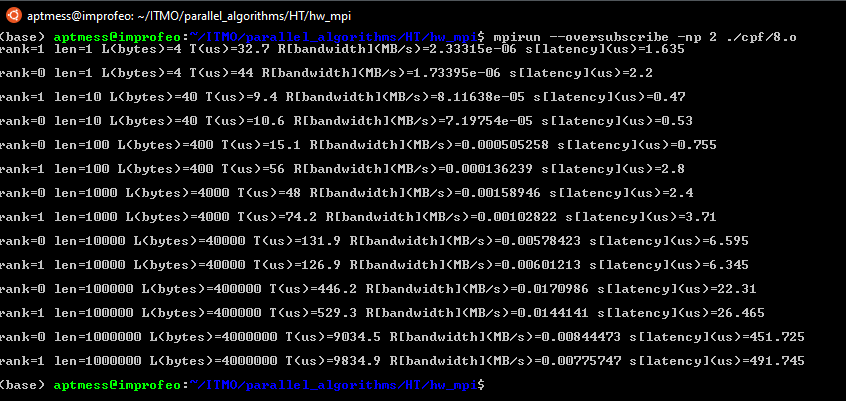
\includegraphics[scale=0.75]{8.png}
% \end{center}

Let's move to the the code and explain how it works.

% \begin{figure}[h!]
% \centering
% \subfigure{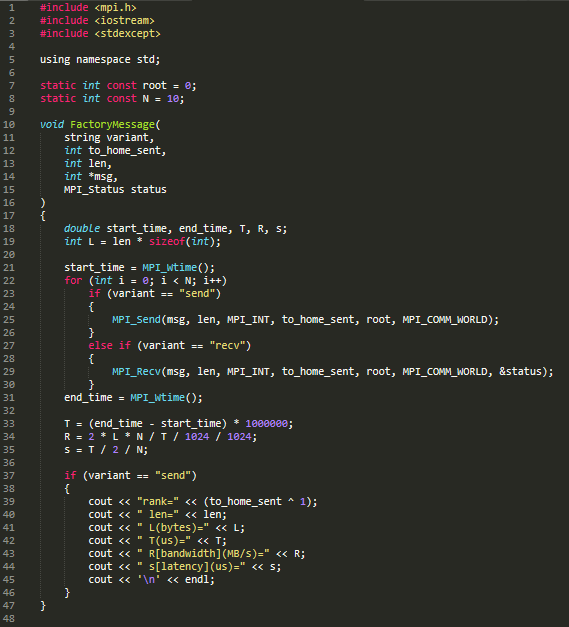
\includegraphics[width=0.47\textwidth]{8.1.code.png}} 
% \subfigure{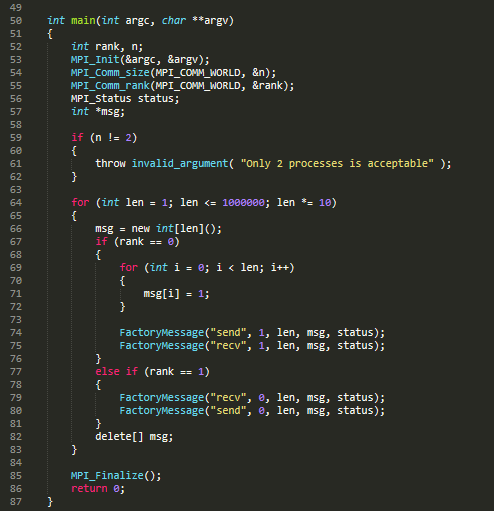
\includegraphics[width=0.5\textwidth]{8.2.code.png}} 

% Assignment8 code
% \end{figure}

\newpage
\subsection{Assignment 10. MPI. Sending and receiving messages without blocking. Ring exchange using non-blocking operations.}

\subsubsection{Formulation of the problem}

Complete the program \textsc{Assignment10.c.} Compile and run it.

Study the code carefully and explain how it works.

\subsubsection{Example of launch parameters and output. Detailed description of solution}

Code for \textbf{assignment 10} is \href{https:\//github.com/aptmess/parallel_algorithms/blob/master/HT/hw_mpi/Assignment10.c}{here}.

Compilation example: \textsc{mpic++ -o ./cpf/10.o Assignment10.c}

Launch example: \textsc{mpirun --oversubscribe -np 10 ./cpf/10.o}

\begin{center}
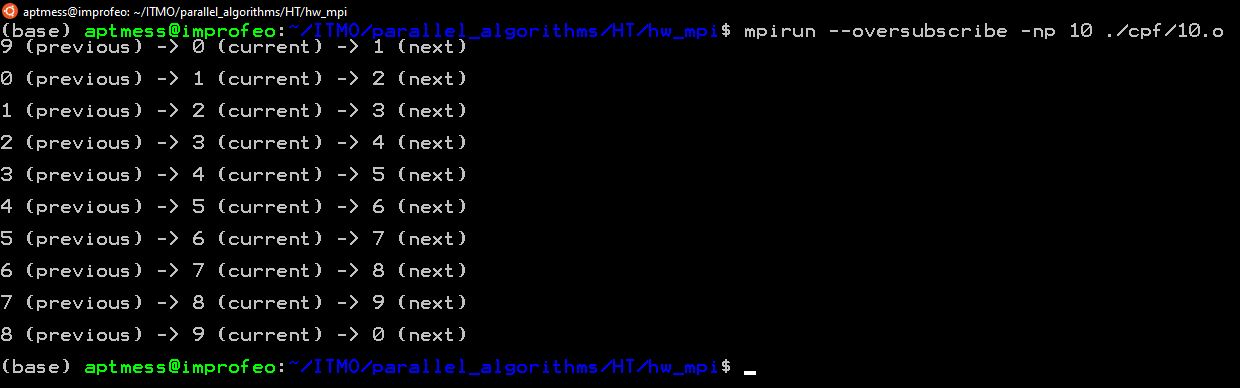
\includegraphics[scale=0.5]{10.png}
\end{center}

Let's move to the the code and explain how it works.

\begin{center}
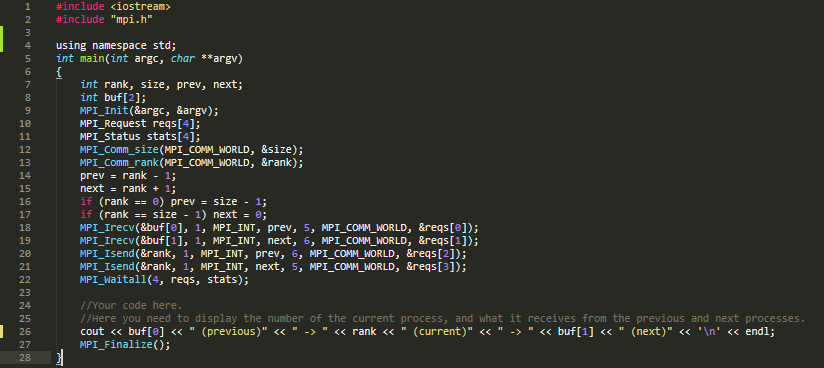
\includegraphics[scale=0.75]{10.code.png}

Assignment 10
\end{center}

The overall goal of the program is that all processes exchange messages with their nearest neighbors (on the left - previous, on the right - next) in accordance with the topology of the ring. Witg \textsc{MPI\_Waitall} the execution of the process is blocked until all exchange operations on the specified \textsc{reqs} identifiers (lines 18-21) are completed and if the error exists in this operations, then the error field in the \textsc{stats} array elements will be set to the appropriate value. In lines $18-21$ there are operations \textsc{MPI\_Irecv} and \textsc{MPI\_Isend} which are equal to previous functions \textsc{MPI\_Recv} and \textsc{MPI\_Send} but in this functions the return from the function occurs immediately after the initialization of the receiving/transmitting process without waiting for the receipt/ processing of the entire message, so we can solve the problem with blocking operations in \textsc{MPI\_Send} and \textsc{MPI\_Recv}. In this lines the process waiting for their neareset neighbours and save information in int array \textsc{buf} and send information about yourself's rank to previous and next. The result is displayed on screens - ring topology works.



\subsection{Appendix}

The link to the sourse code which is placed on my \href{https://github.com/aptmess/parallel_algorithms}{github}.


\end{document}